\documentclass[11pt, a4paper]{article}
%\usepackage{proj1}
\usepackage{natbib}
\usepackage{fancyhdr}  
\usepackage{subcaption}
\usepackage{caption}
\usepackage{graphicx}
\linespread{1.25} 
\setlength{\parindent}{0cm}
\graphicspath{{Images/}}
\usepackage{hyperref}
\usepackage{amsmath}
\usepackage{amsfonts}
\usepackage{amssymb}
\usepackage{amsthm}
\usepackage{mathtools}
\usepackage{commath}

%\usepackage[sc,osf]{mathpazo}
\usepackage{subcaption}
\usepackage[a4paper, top=1in, left=1.0in, right=1.0in, bottom=1in, includehead, includefoot]{geometry} %Usually have top as 1in

\usepackage{listings}
\usepackage{color} %red, green, blue, yellow, cyan, magenta, black, white
\definecolor{mygreen}{RGB}{28,172,0} % color values Red, Green, Blue
\definecolor{mylilas}{RGB}{170,55,241}


\hypersetup{colorlinks,linkcolor={black},citecolor={blue},urlcolor={black}}
\usepackage{color}
\urlstyle{same}


\theoremstyle{definition}
\newtheorem{definition}{Definition}[section]

\title{Exact Solutions for the Full Problem \\with Force Control and with Flow Control}
\date{}
\newcommand{\Sta}{\rho}
\newcommand{\Adj}{p}
\newcommand{\Con}{u}

\pagenumbering{gobble}
\begin{document}
\section*{Report 23/04/2020}
Quick observation: When relaxing the tolerances, we need to check the exact solutions. For example in FixPt, when we set the ODE tolerance to $10^{-7}$, the consistency error in $w$ is larger than $10^{-4}$, so we need to adapt that. This is less of an issue in the way that Multiple Shooting consistency errors are calculated because they are added and not multiplied.
\\
\\
Generally we will have $n=61$, $N=60$, ODE Tols = $10^{-8}$, Consistency Tols = $10^{-4}$, $\lambda = 0.01$, solver FixPt and $\gamma = 1$ repulsive, $\gamma = -1$ attractive.
\section{Interacting Problems - static target 1}
The considered problem is the following:
\begin{align*}
\partial_t \rho = D_0\Delta \rho - \nabla \cdot (\rho w) + \gamma \nabla \cdot \int_\Omega \rho \rho' \nabla V_2 dr,
\end{align*}
with $w =0$ in the forward case, but flow control in the optimization problem. There is no force term involved and mass is conserved.
The initial condition for $\rho$ is:
\begin{align*}
\rho_{IC} = 0.5,
\end{align*}
such that $\int_{-1}^{1}\rho_{IC} = 1$.
The first choice of $\hat \rho$ is:
\begin{align*}
&\hat \rho = \frac{1}{4}\cos(\pi y +\pi) + \frac{1}{2}\\
&\int_{-1}^{1}\frac{1}{4}\cos(\pi y + \pi) + \frac{1}{2}dy =1,
\end{align*}
see Figure \ref{rhoTarget1}.
\begin{figure}[h]
	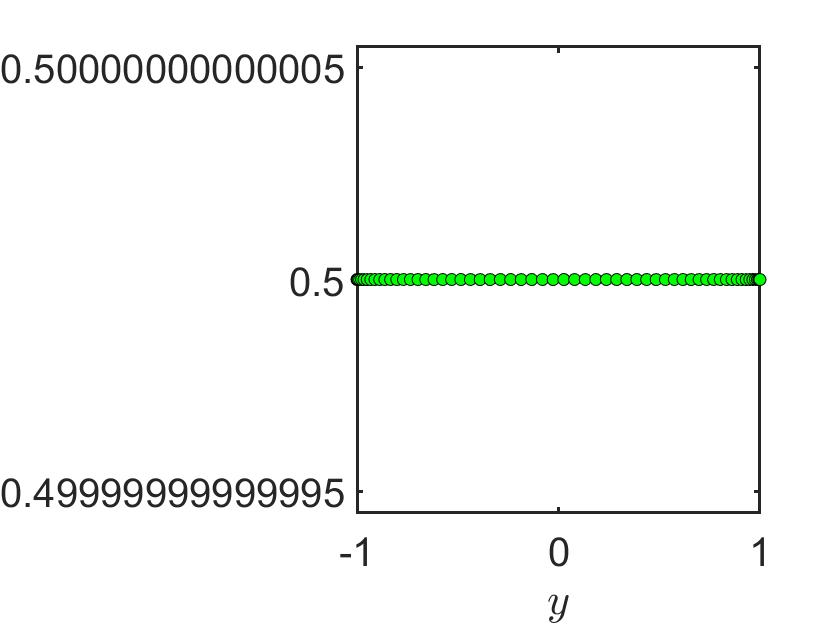
\includegraphics[scale=0.3]{rhoIC1.jpg}
	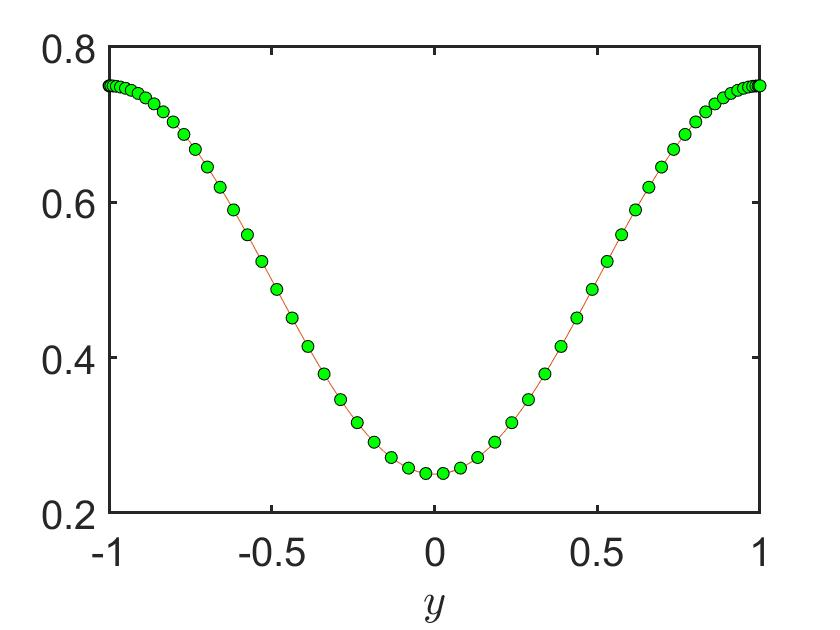
\includegraphics[scale=0.3]{rhoHat1.jpg}
	\caption{First Choice of $\rho_{IC}$ and $\hat \rho$.}
	\label{rhoTarget1}
\end{figure}

Using 'FixPt' and looking at $\beta = 10^{-1}$ we get the following results:
First consider $\gamma = 1$.
Then the forward and optimal solutions can be seen in Figure \ref{rho01}. The optimal control can also be seen in Figure \ref{rho01}. $J_{FW} = 0.0193$ and $J_{Opt} = 0.0164$.\\
For $\gamma = -1$, the situation is a little different, see Figure \ref{rho01a}. When $\gamma =1$, the interaction is driving towards the desired state, when $\gamma = -1$, it is driving away from it. $J_{FW} = 0.0488$ and $J_{Opt}= 0.0392$.\\
When setting $\beta = 10$ for both $\gamma =1$ and $\gamma =-1$, the algorithm solves the problem in $300$ to $400$ iterations ($\beta = 10^{-1}$ needs $700$ to $800$ iterations). Then $J$ is more or less the same in the forward and optimal case, as expected.\\
The case $\beta = 10^{-3}$ is a bit more tricky. Both for $\gamma = 1$ and $\gamma = -1$, the algorithm diverges.\\
Choose $\gamma = 0.5$ and $\beta = 10^{-3}$, then it diverges at $0.00061179$, however, while $J_{FW} = 0.0247$, $J_{Opt} = 0.0019$, so the overall cost is already lowered, see Figure \ref{rho00305a}.
Choosing $\gamma = -0.5$, the algorithm diverges at $0.00055109$, however, the solution is already improved, $J_{FW} = 0.0329$, $J_{Opt} = 0.0023$, see Figure \ref{rho00305}.
The two figures (\ref{rho00305a} and \ref{rho00305}) look very similar.\\
My theory is that for small $\beta$, the advection term is allowed to get very large, which causes problems for the solution of the equation. Looking at Figures \ref{rho00305} and \ref{rho00305a} seem to confirm this: While $\rho$ is around $0.5$, $w$ is around $10$.


\begin{figure}[h]
	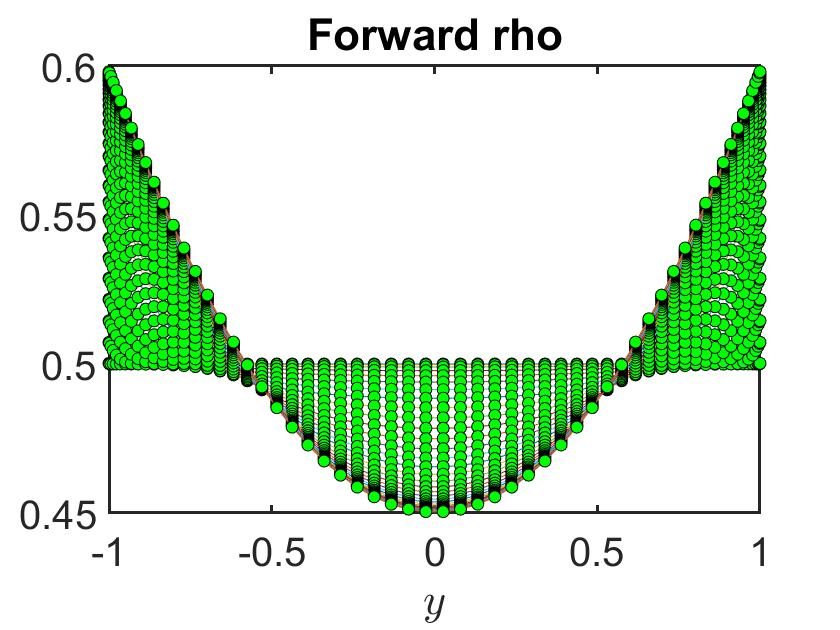
\includegraphics[scale=0.3]{rhoFW01.jpg}
	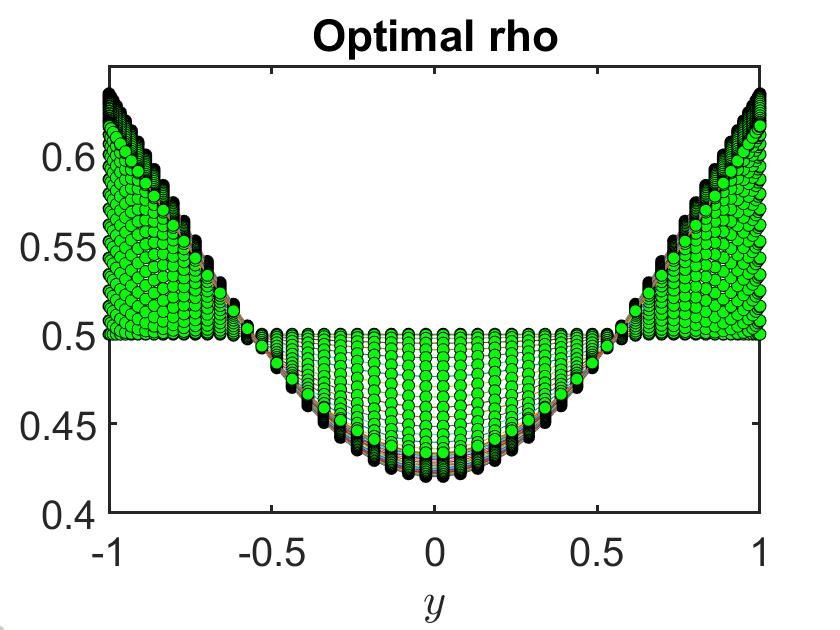
\includegraphics[scale=0.3]{rhoOpt01.jpg}
	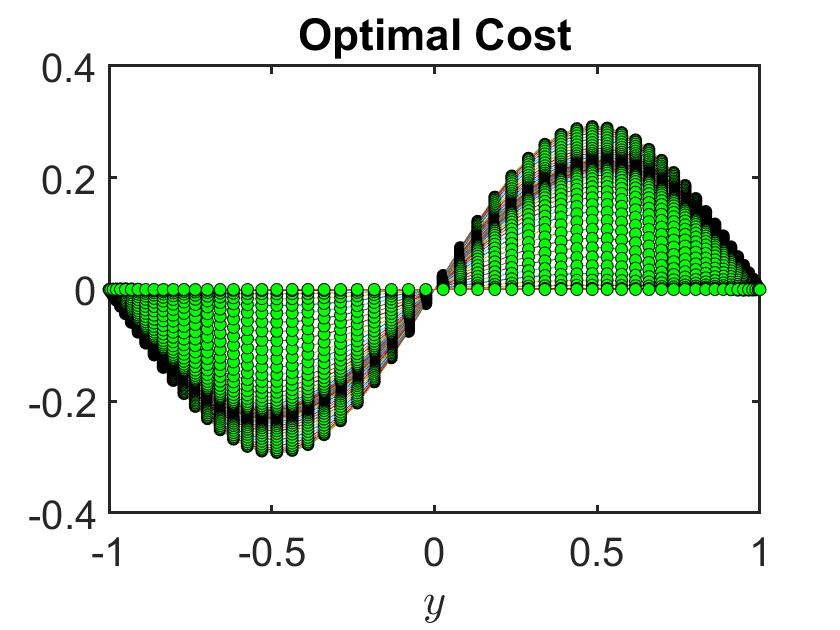
\includegraphics[scale=0.3]{wOpt01.jpg}
	\caption{Solutions $\rho_{FW}$ and $\rho_{Opt}$ and Optimal control $w$, $\gamma = 1$, $\beta = 10^{-1}$.}
	\label{rho01}
\end{figure}

\begin{figure}[h]
	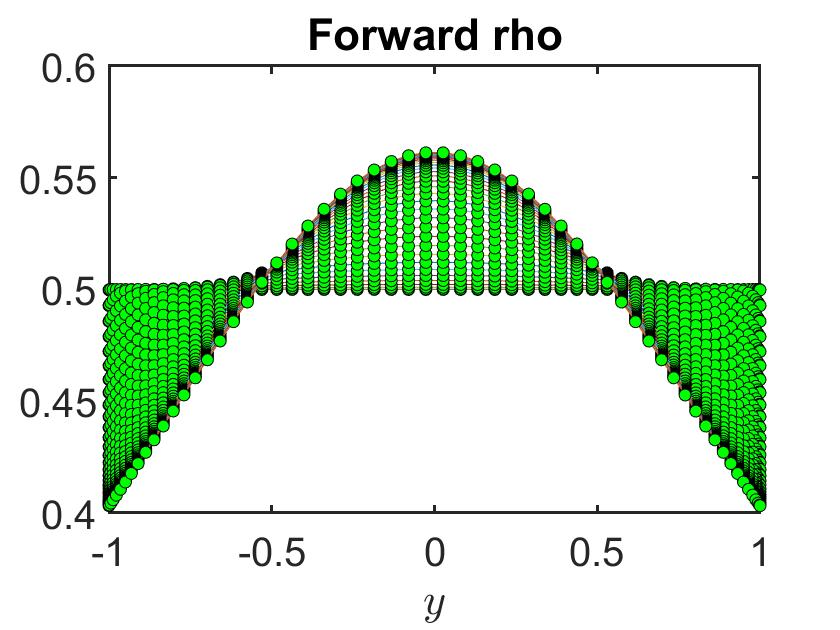
\includegraphics[scale=0.3]{rhoFW01a.jpg}
	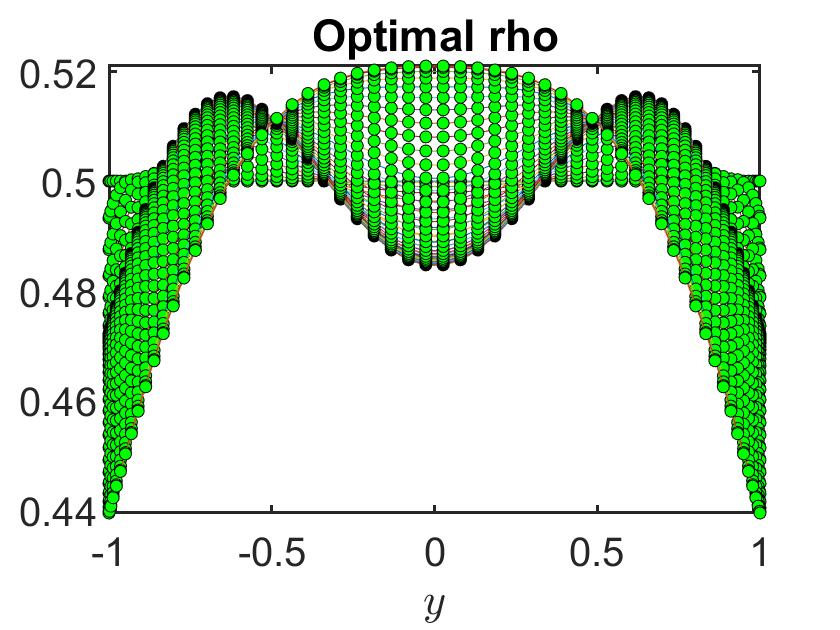
\includegraphics[scale=0.3]{rhoOpt01a.jpg}
	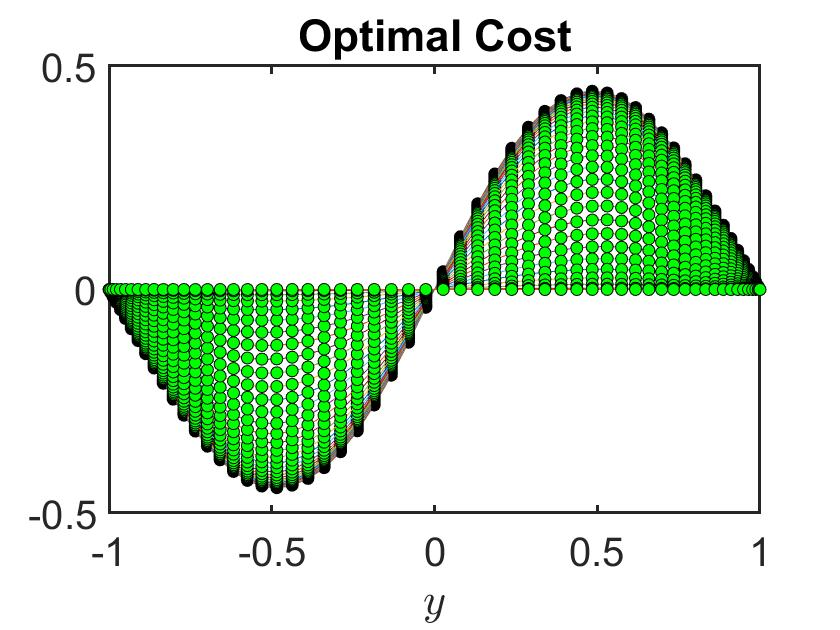
\includegraphics[scale=0.3]{wOpt01a.jpg}
	\caption{Solutions $\rho_{FW}$ and $\rho_{Opt}$ and Optimal control $w$, $\gamma = - 1$, $\beta = 10^{-1}$.}
	\label{rho01a}
\end{figure}
\begin{figure}[h]
	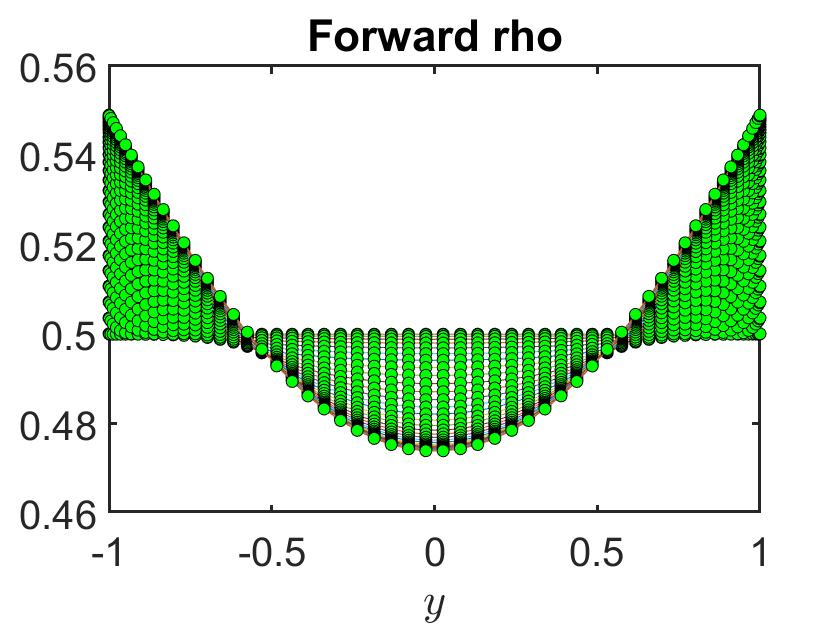
\includegraphics[scale=0.3]{rhoFW0305a.jpg}
	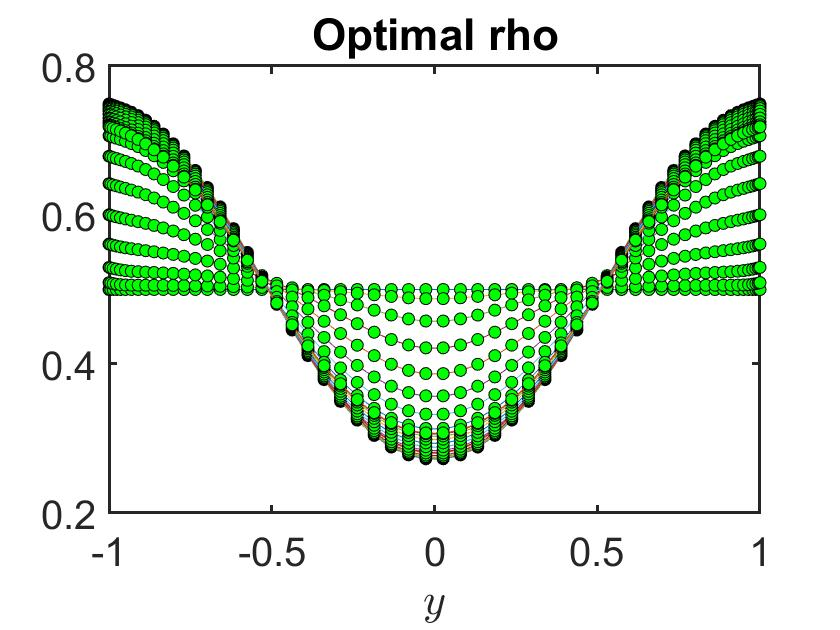
\includegraphics[scale=0.3]{rhoOpt0305a.jpg}
	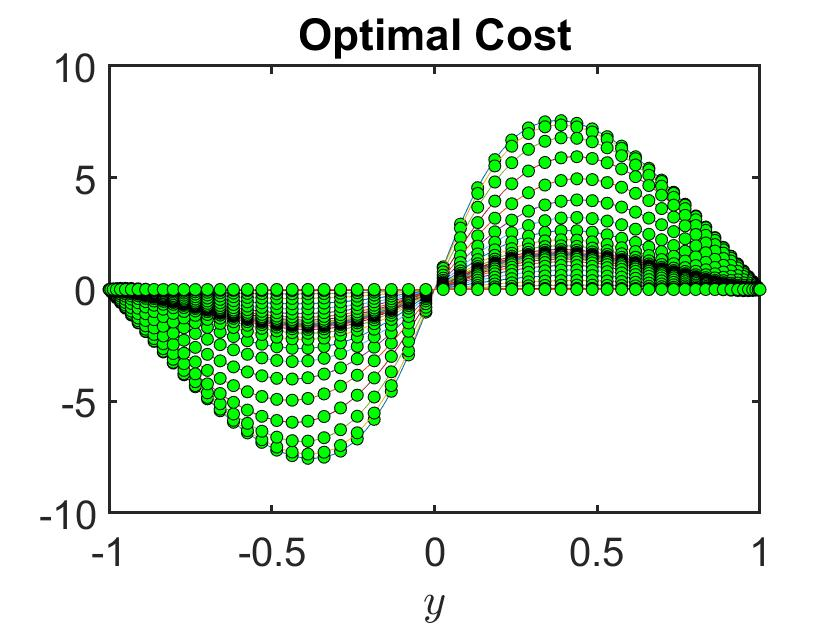
\includegraphics[scale=0.3]{wOpt0305a.jpg}
	\caption{Solutions $\rho_{FW}$ and $\rho_{Opt}$ and Optimal control $w$, $\gamma = 0.5$, $\beta = 10^{-3}$.}
	\label{rho00305a}
\end{figure}

\begin{figure}[h]
	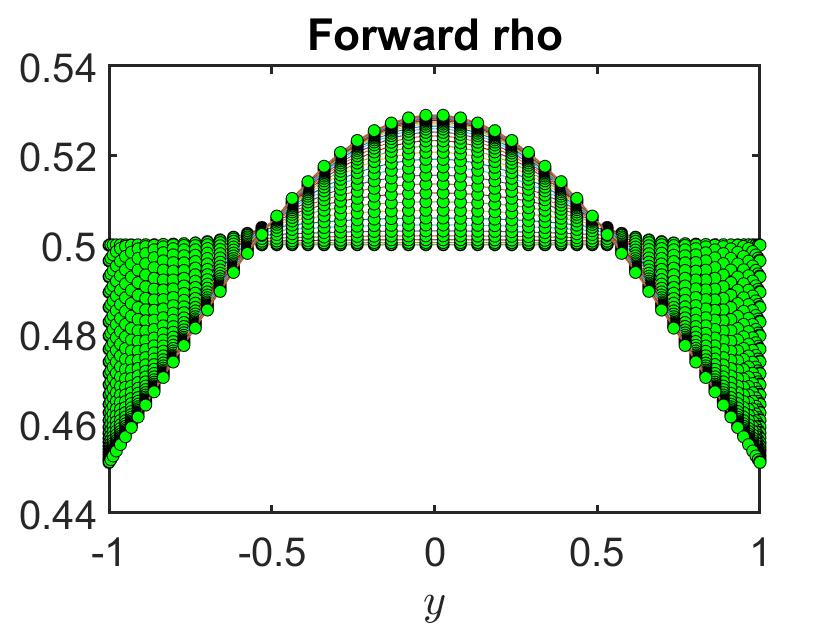
\includegraphics[scale=0.3]{rhoFW0305.jpg}
	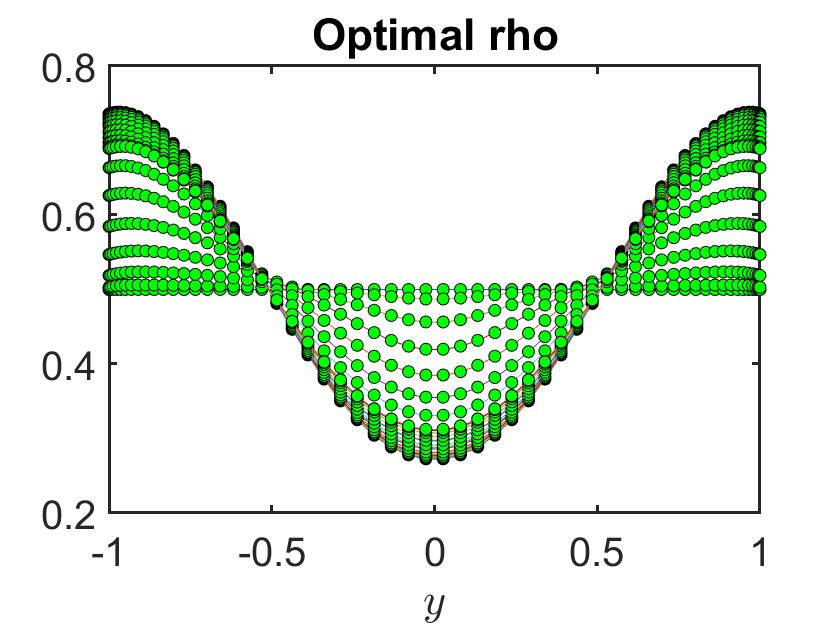
\includegraphics[scale=0.3]{wOpt0305.jpg}
	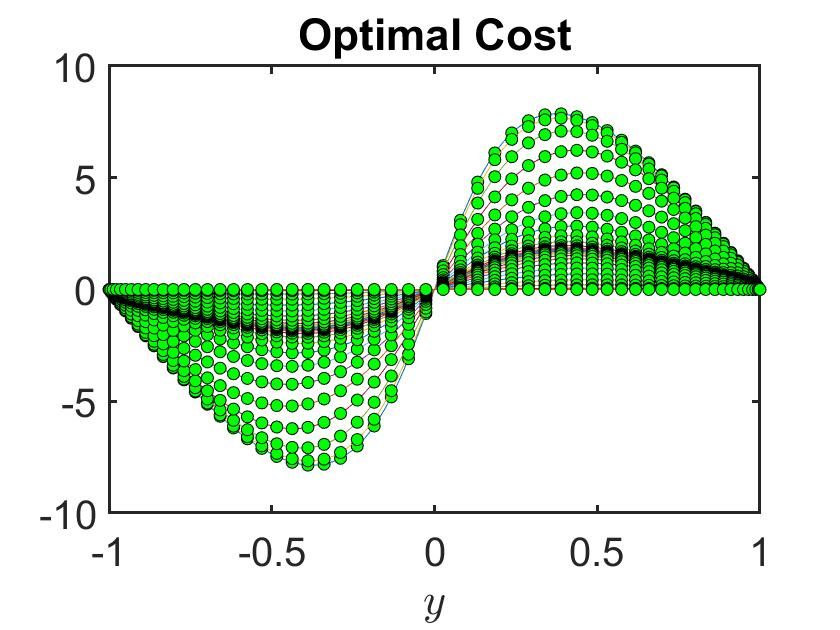
\includegraphics[scale=0.3]{rhoOpt0305.jpg}
	\caption{Solutions $\rho_{FW}$ and $\rho_{Opt}$ and Optimal control $w$, $\gamma = - 0.5$, $\beta = 10^{-3}$.}
	\label{rho00305}
\end{figure}

\subsection{Diffusion vs advection term}
If we change the diffusion coefficient in this problem, we can see whether this theory is true.
Changing $D_0$ to $2$, for $\gamma = - 0.5$, shows that it now diverges at $0.00011836$. This is a bit later than before. When we choose $D_0 = 3$, the problem converges, with $J_{FW} = 0.0339$, $J_{Opt}= 0.0096$ within $787$ iterations, see Figure \ref{rho00305D03}.\\
The same thing works for $\gamma = 0.5$, $J_{FW} = 0.0287$ and $J_{Opt} = 0.0085$, see Figure \ref{rho00305D03a}. In fact $\gamma = -1$ converges with $D_0 =2$, but $\gamma = 1$ diverges with $D_0 = 2$, but converges with $D_0=5$. I conclude that the issue of convergence has to do with the strength of the advection term in comparison to the other terms in the equation.
\begin{figure}[h]
	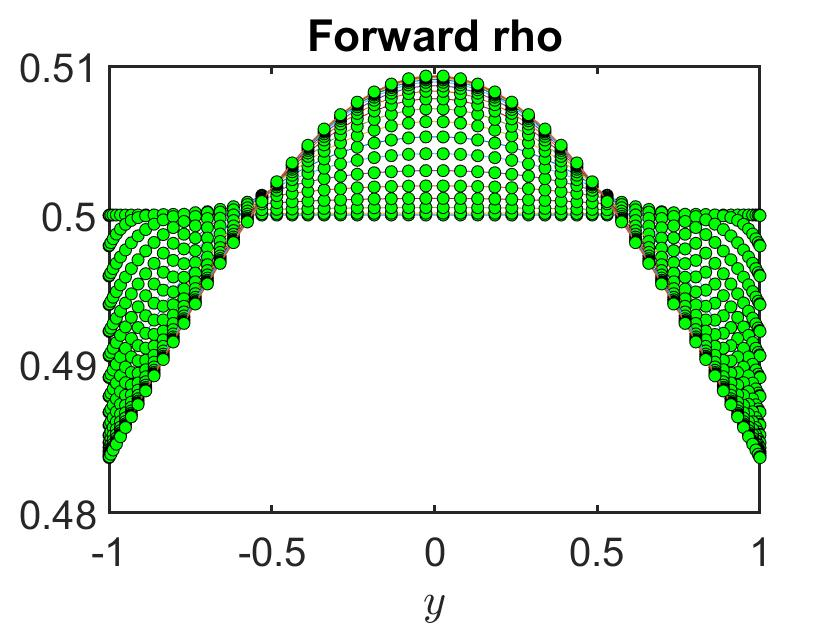
\includegraphics[scale=0.3]{rhoFW0305D03.jpg}	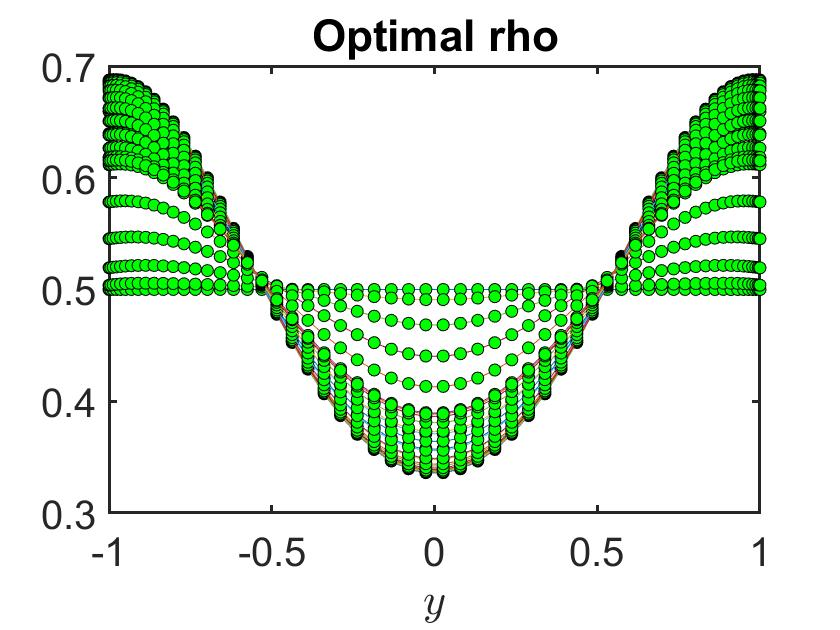
\includegraphics[scale=0.3]{rhoOpt0305D03.jpg}
	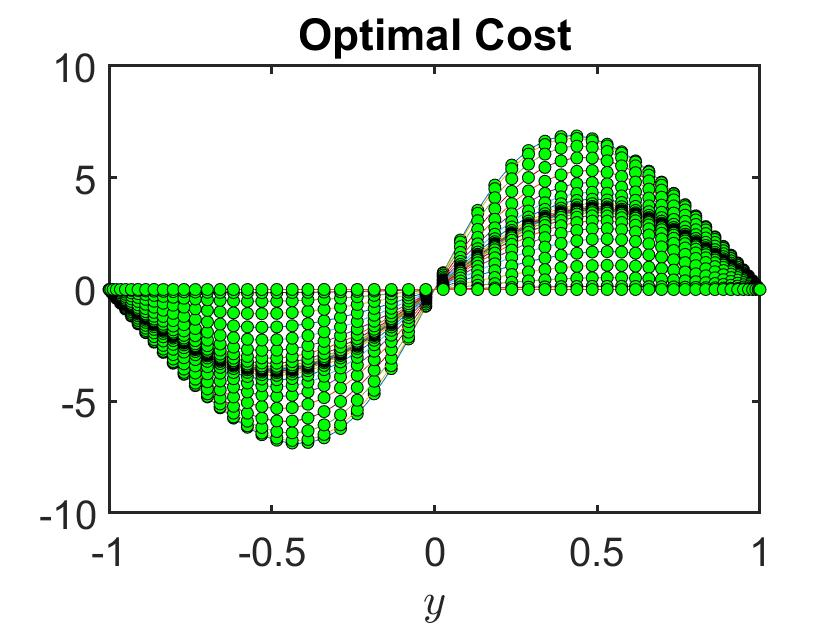
\includegraphics[scale=0.3]{wOpt0305D03.jpg}
	\caption{Solutions $\rho_{FW}$ and $\rho_{Opt}$ and Optimal control $w$, $\gamma = - 0.5$, $\beta = 10^{-3}$, with $D_0 = 3$.}
	\label{rho00305D03}
\end{figure}

\begin{figure}[h]
	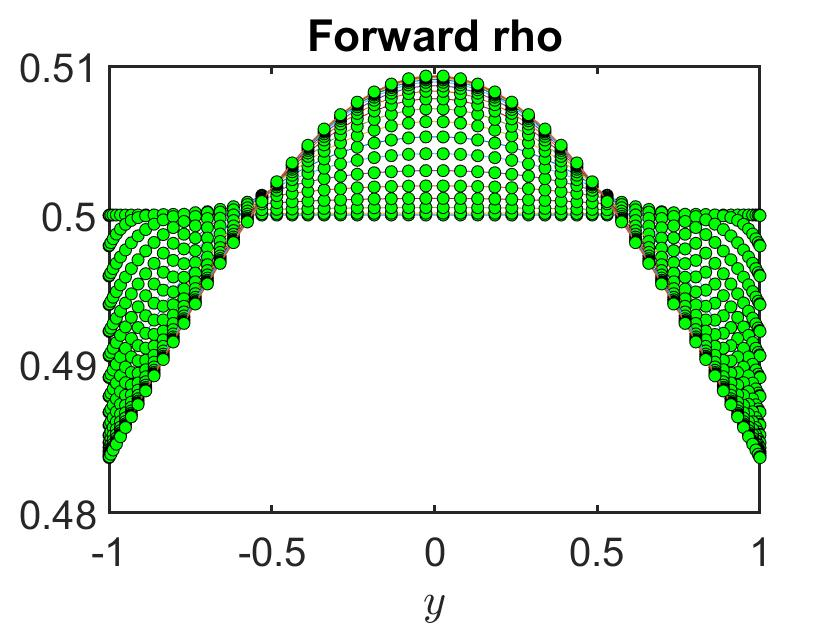
\includegraphics[scale=0.3]{rhoFW0305D03.jpg}	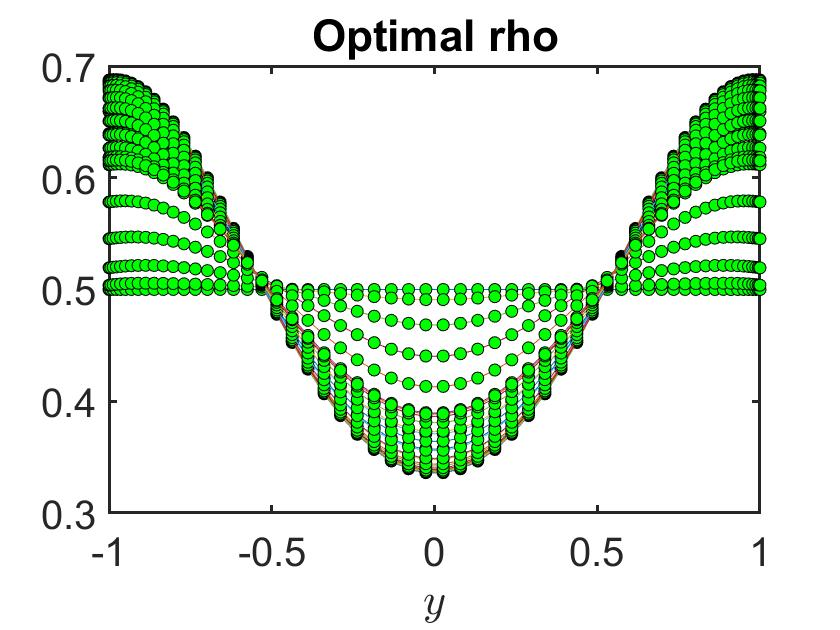
\includegraphics[scale=0.3]{rhoOpt0305D03.jpg}
	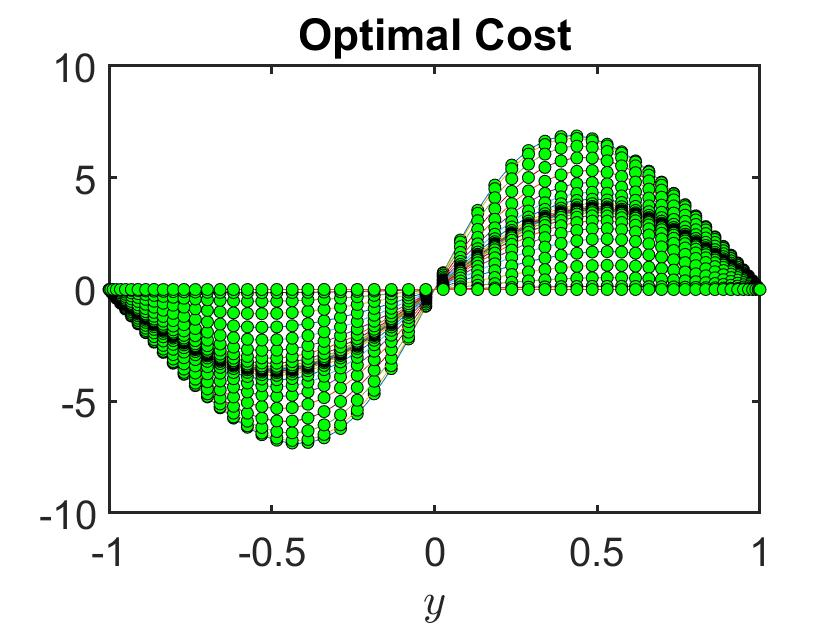
\includegraphics[scale=0.3]{wOpt0305D03.jpg}
	\caption{Solutions $\rho_{FW}$ and $\rho_{Opt}$ and Optimal control $w$, $\gamma = - 0.5$, $\beta = 10^{-3}$, with $D_0 = 3$.}
	\label{rho00305D03a}
\end{figure}

\section{Interacting Problems - static target 2}
Investigating a similar problem but this time the target is:
\begin{align*}
&\hat \rho = \frac{1}{4}\cos(\pi y) + \frac{1}{2}\\
&\int_{-1}^{1}\frac{1}{4}\cos(\pi y) + \frac{1}{2}dy =1,
\end{align*}
so that the particles are supposed to go to the middle, see Figure \ref{rhoHat2}.
\begin{figure}[h]
	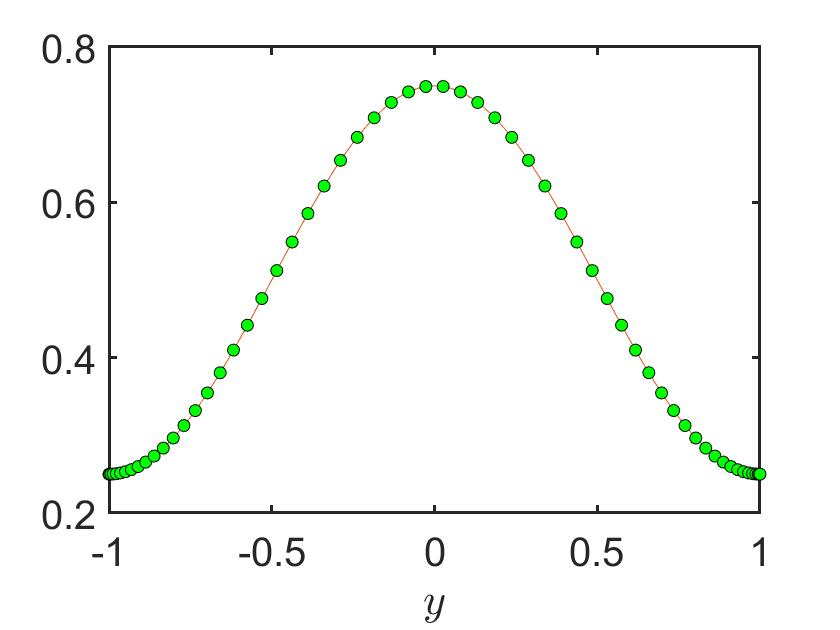
\includegraphics[scale=0.3]{rhoHat2.jpg}	
	\caption{$\hat \rho$ 2.}
	\label{rhoHat2}
\end{figure}

Starting with $\beta = 10^{-1}$ and $\gamma = - 1$, we have $J_{FW}= 0.0179$ and $J_{Opt}=0.0146$, see Figure \ref{rhoD01}. As expected, in comparison to the other example, $w$ is pushing the solution inwards (while in the above example, it pushed the particles outwards).With $\gamma = 1$, $J_{FW}= 0.0466$ and $J_{Opt} = 0.032$, see Figure \ref{rhoD01a}. We can observe that the order of magnitude of $w$ is around the same for both $\gamma$ (restricted by J/ $\beta$?), but the results aren't as close to $\hat \rho$, since the interactions are working against the target (interactions repulsive).\\
Checking $\beta = 10^{-3}$ next, expecting a similar result as above. As expected, the case with $\gamma = - 1$ diverges at $0.00051689$. $J_{FW}= 0.0179$ and $J_{Opt}= 0.0013$, see Figure \ref{rhoD03a}. Choosing $\gamma = 1$ surprisingly converges in $778$ iterations. $J_{FW} = 0.0466$, $J_{Opt} = 0.0031$, see Figure \ref{rhoD03}. It is especially surprising given that the particle interactions are repulsive, while the target is in the middle of the domain. A theory could be that the particle interaction is in the 'opposite direction' to the advection and therefore it isn't as advection dominated as the problem with attractive particles?\\
Checked both $\gamma =1$ and $\gamma = -1$ with $\beta = 10$, which converges and doesn't seem to pose a problem.

\begin{figure}[h]
	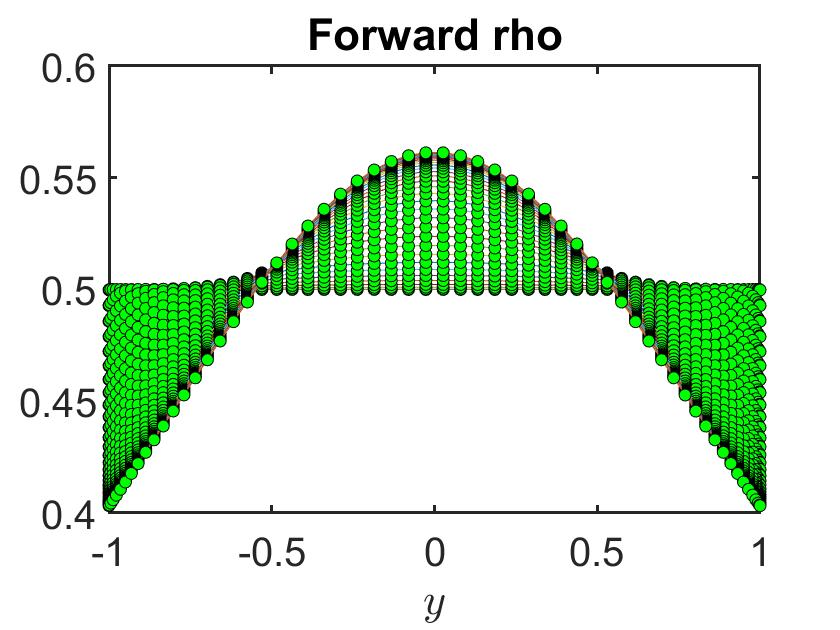
\includegraphics[scale=0.3]{rhoFWD01.jpg}	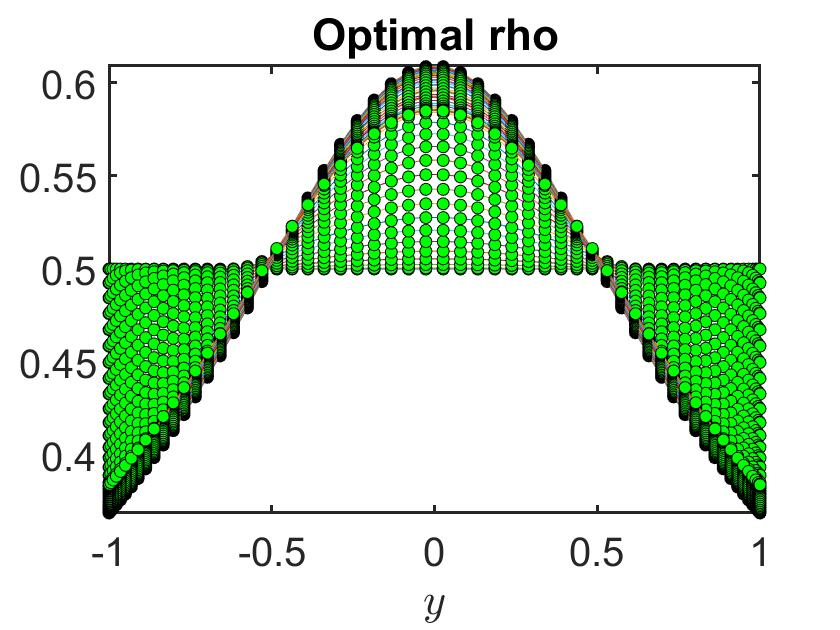
\includegraphics[scale=0.3]{rhoOptD01.jpg}
	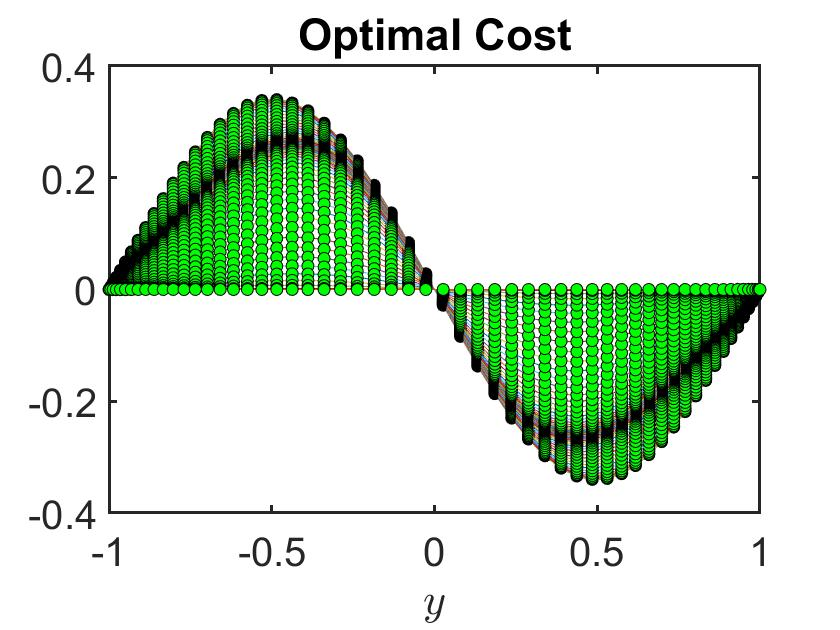
\includegraphics[scale=0.3]{wOptD01.jpg}
	\caption{Solutions $\rho_{FW}$ and $\rho_{Opt}$ and Optimal control $w$, $\gamma = - 1$, $\beta = 10^{-1}$, with $D_0 = 1$.}
	\label{rhoD01}
\end{figure}
\begin{figure}[h]
	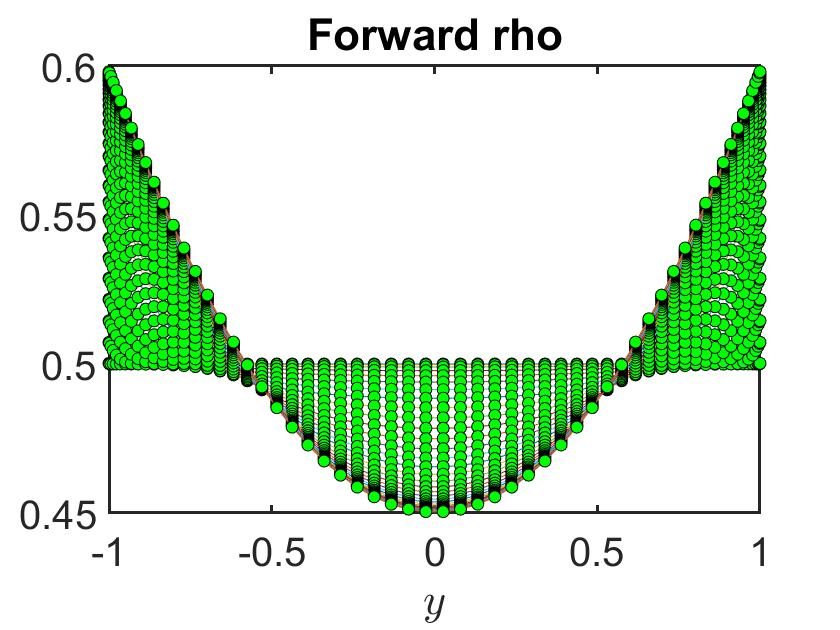
\includegraphics[scale=0.3]{rhoFWD01a.jpg}	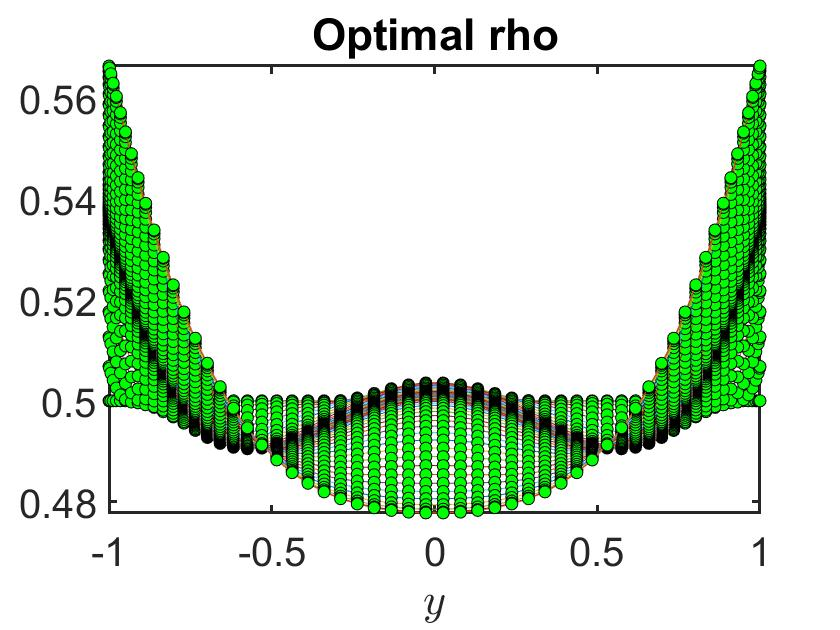
\includegraphics[scale=0.3]{rhoOptD01a.jpg}
	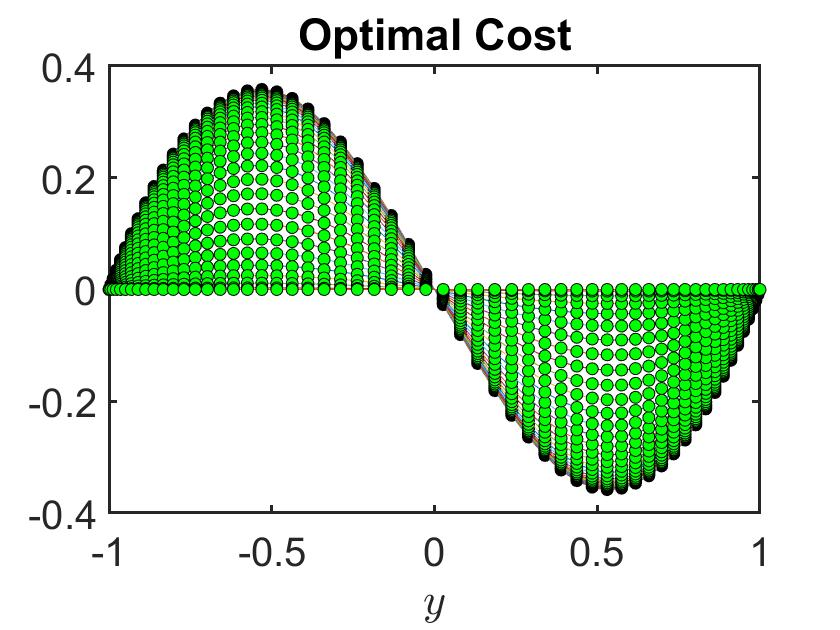
\includegraphics[scale=0.3]{wOptD01a.jpg}
	\caption{Solutions $\rho_{FW}$ and $\rho_{Opt}$ and Optimal control $w$, $\gamma = 1$, $\beta = 10^{-1}$, with $D_0 = 1$.}
	\label{rhoD01a}
\end{figure}
\begin{figure}[h]
	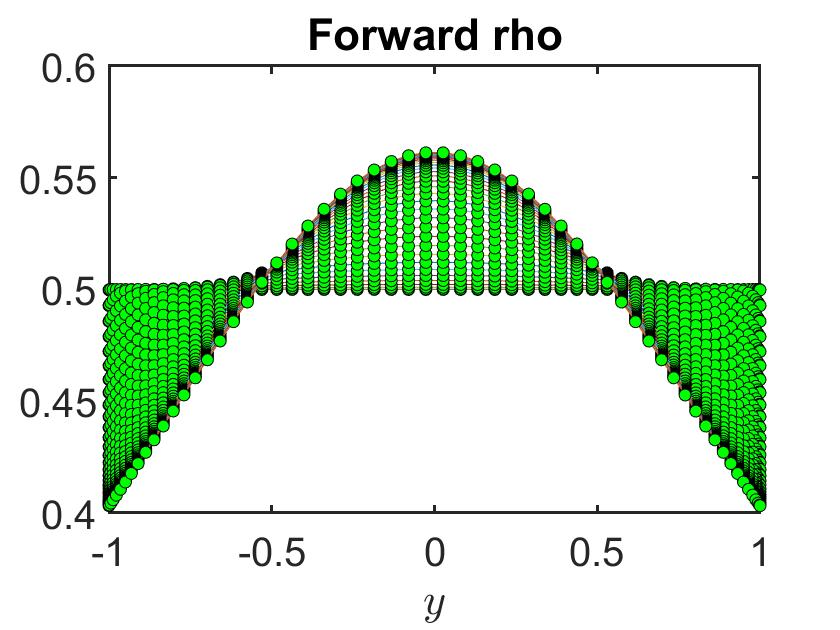
\includegraphics[scale=0.3]{rhoFWD03a.jpg}	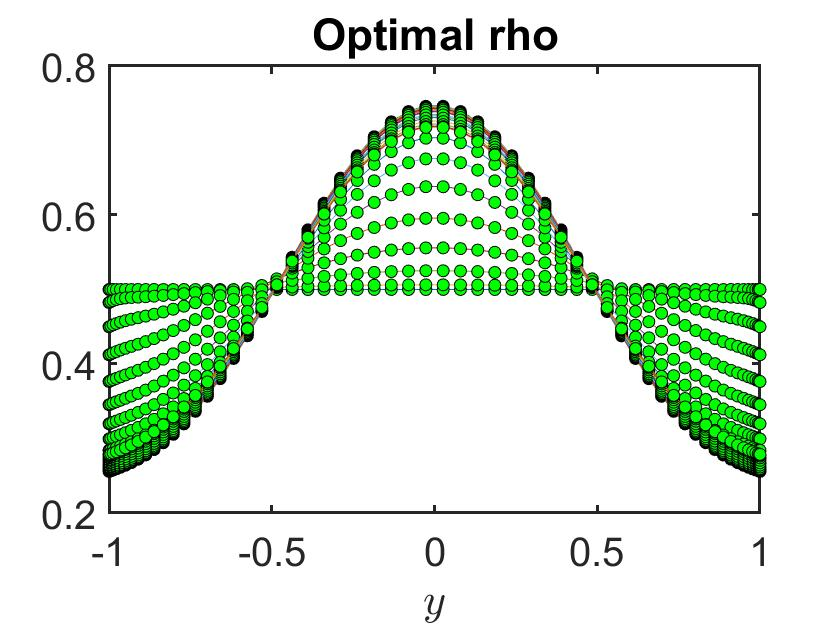
\includegraphics[scale=0.3]{rhoOptD03a.jpg}
	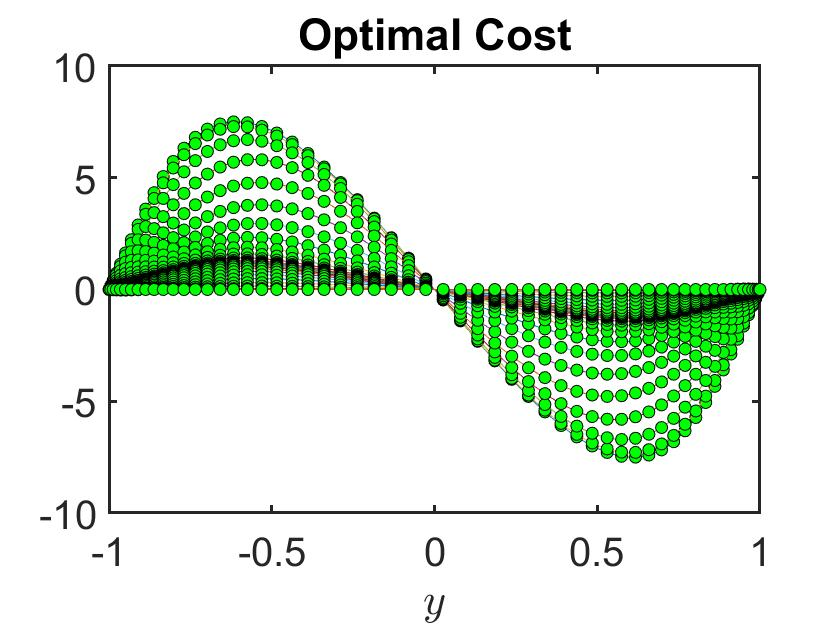
\includegraphics[scale=0.3]{wOptD03a.jpg}
	\caption{Solutions $\rho_{FW}$ and $\rho_{Opt}$ and Optimal control $w$, $\gamma = - 1$, $\beta = 10^{-3}$, with $D_0 = 1$.}
	\label{rhoD03a}
\end{figure}
\begin{figure}[h]
	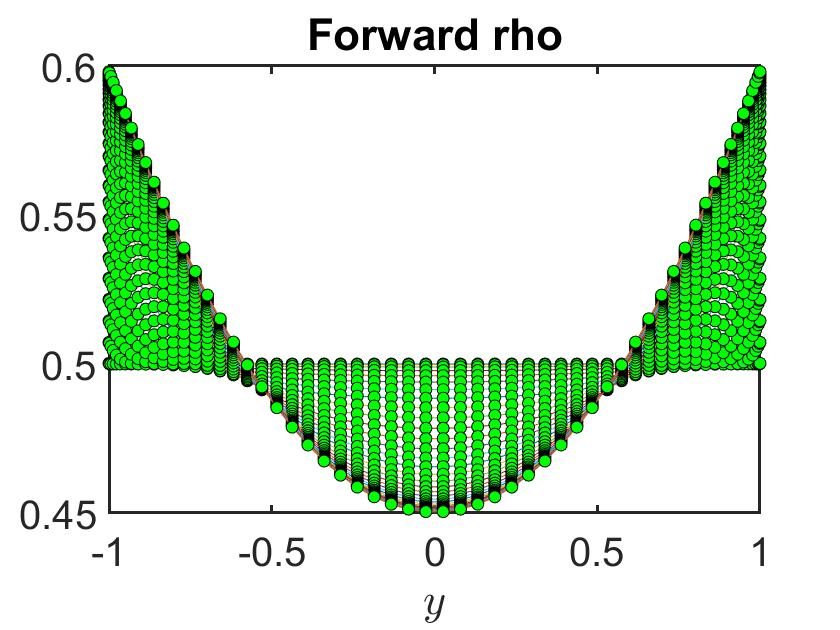
\includegraphics[scale=0.3]{rhoFWD03.jpg}	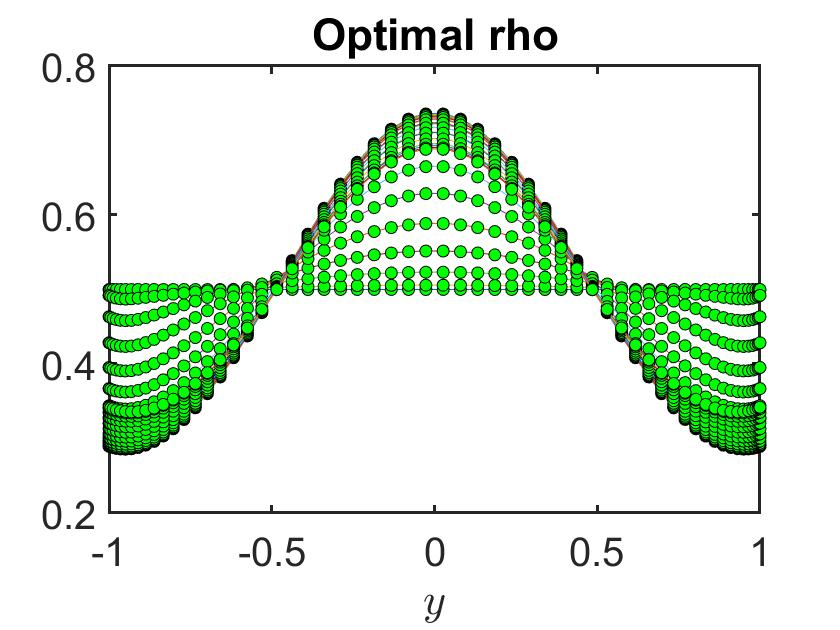
\includegraphics[scale=0.3]{rhoOptD03.jpg}
	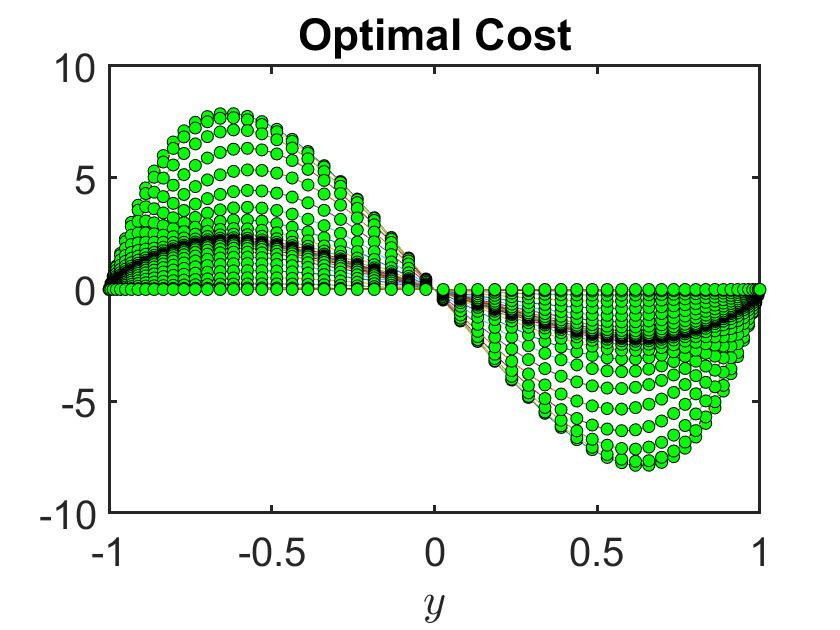
\includegraphics[scale=0.3]{wOptD03.jpg}
	\caption{Solutions $\rho_{FW}$ and $\rho_{Opt}$ and Optimal control $w$, $\gamma = 1$, $\beta = 10^{-3}$, with $D_0 = 1$.}
	\label{rhoD03}
\end{figure}
\subsection{Diffusion vs advection term}
As for the other example, we can try to increase the diffusion to confirm that a large advection term is the problem. Choosing $\beta = 10^{-3}$, $\gamma = -1$ and $D_0 = 3$. This converges in $789$ iterations, $J_{FW} = 0.0262$ and $J_{Opt} = 0.0074$, see Figure \ref{rhoD03D3}. We can conclude that this again is an issue of advection dominance. However, it is interesting that the $\gamma = 1$ case worked for $D_0 = 1$.
	\begin{figure}[h]
		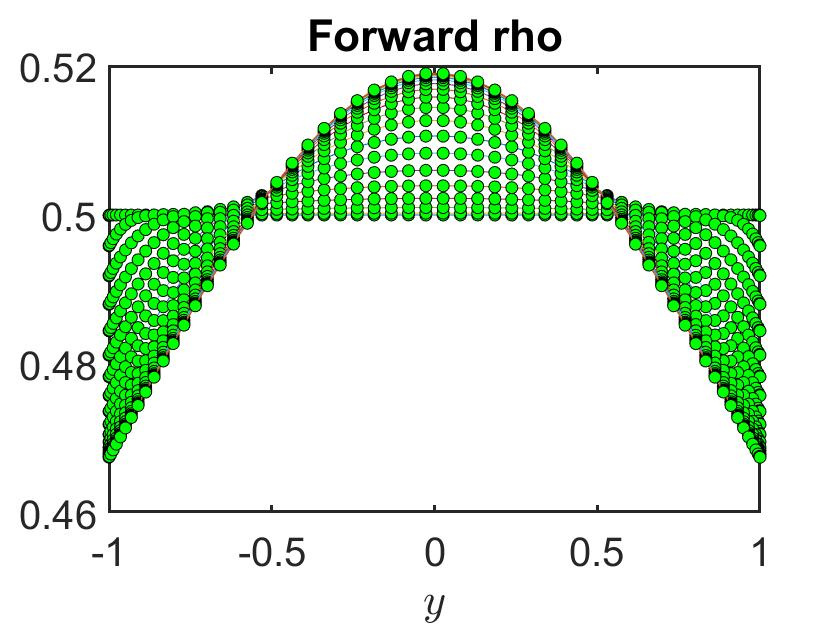
\includegraphics[scale=0.3]{rhoFW03D3.jpg}	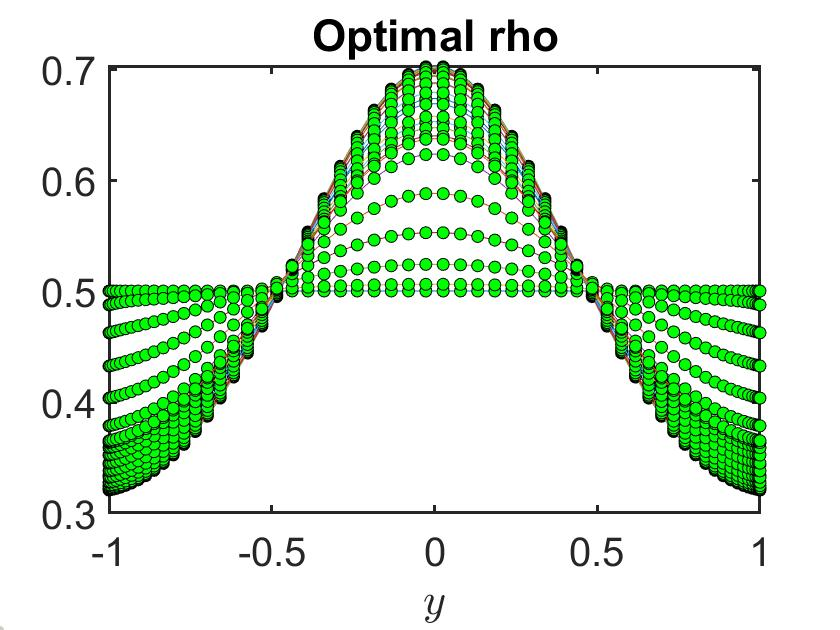
\includegraphics[scale=0.3]{rhoOptD03D3.jpg}
		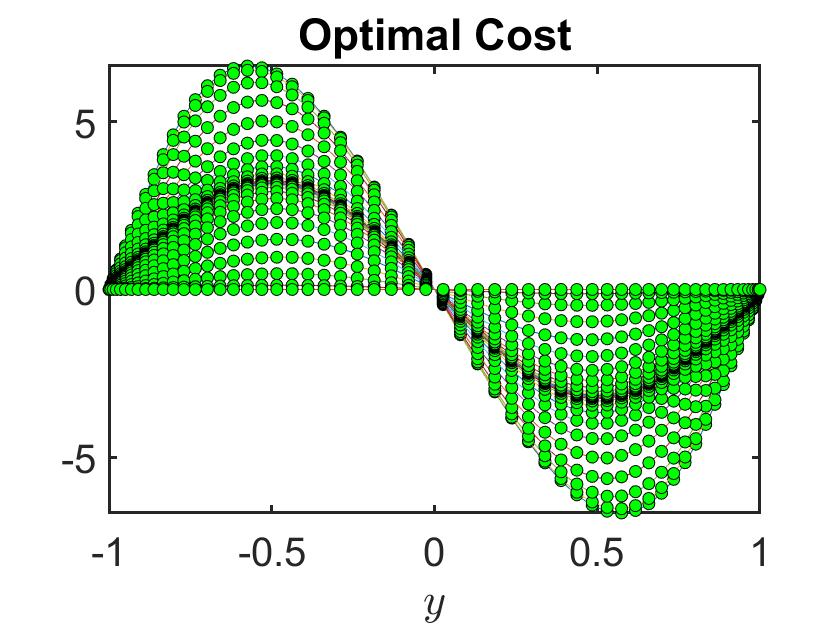
\includegraphics[scale=0.3]{wOpt03D3.jpg}
		\caption{Solutions $\rho_{FW}$ and $\rho_{Opt}$ and Optimal control $w$, $\gamma = - 1$, $\beta = 10^{-3}$, with $D_0 = 3$.}
		\label{rhoD03D3}
	\end{figure}

\section{Interacting Problems - moving target 1}
The target is now
\begin{align*}
\hat \rho = (1-t)0.5 + t\frac{1}{4}(\cos(\pi y) + 2),
\end{align*}
see Figure \ref{rhoHat3}.

\begin{figure}[h]
	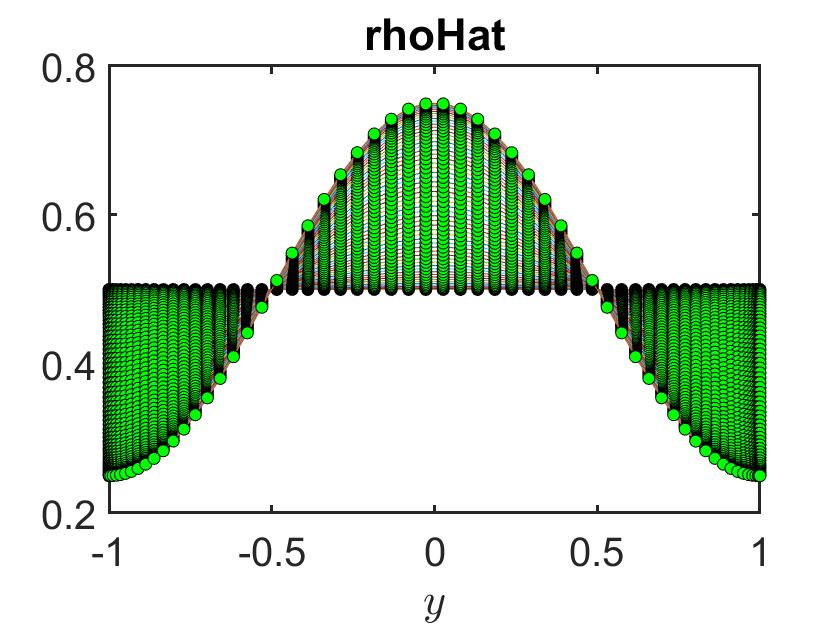
\includegraphics[scale=0.3]{rhoHat3.jpg}
	\caption{Moving target 1.}
	\label{rhoHat3}
\end{figure}

Choosing $\beta = 10^{-1}$, $ \gamma = - 1$, $D_0 = 1$, this converges in $637$ iterations, $J_{FW} = 0.0041$ and $J_{Opt} = 0.0033$. Choosing $\gamma = 1$ also converges with $J_{FW} = 0.0195$ and $J_{Opt} = 0.0164$.\\
Try $\beta = 10$, converges for both $\gamma =1$, $\gamma = -1$, $J_{FW}$ and $J_{Opt}$ basically identical. As perhaps expected, $\beta = 10^3$ converges within one iteration for both choices of $\gamma$.\\
Setting $\beta = 10^{-3}$, $\gamma = 1$, the algorithm converges as well, $J_{FW}= 0.0195$, $J_{Opt} = 0.0011$. Choosing $\gamma = -1$ diverges at $0.00011435$, $J_{FW} = 0.0041$, $J_{Opt}=2.1312 \times 10^{-4}$, see Figure \ref{rhoM1}. This is the same observation as above, advection and interaction work in the same direction, so it is a harder problem?
Choosing $\gamma = - 0.9$ instead of $\gamma = -1$ converges, $J_{FW} = 0.0045$, $J_{Opt} = 2.3514 \times 10^{-4}$. 
\begin{figure}[h]
	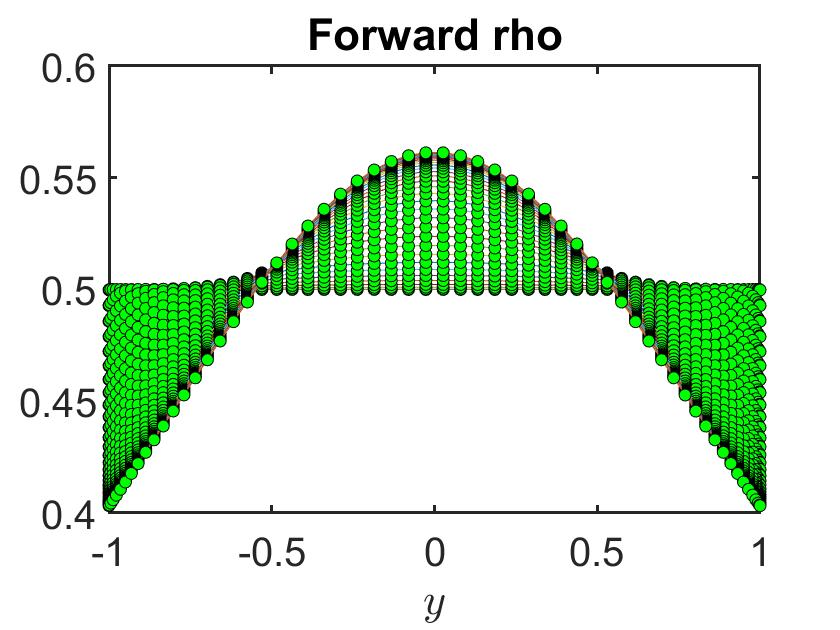
\includegraphics[scale=0.3]{rhoFWM2.jpg}	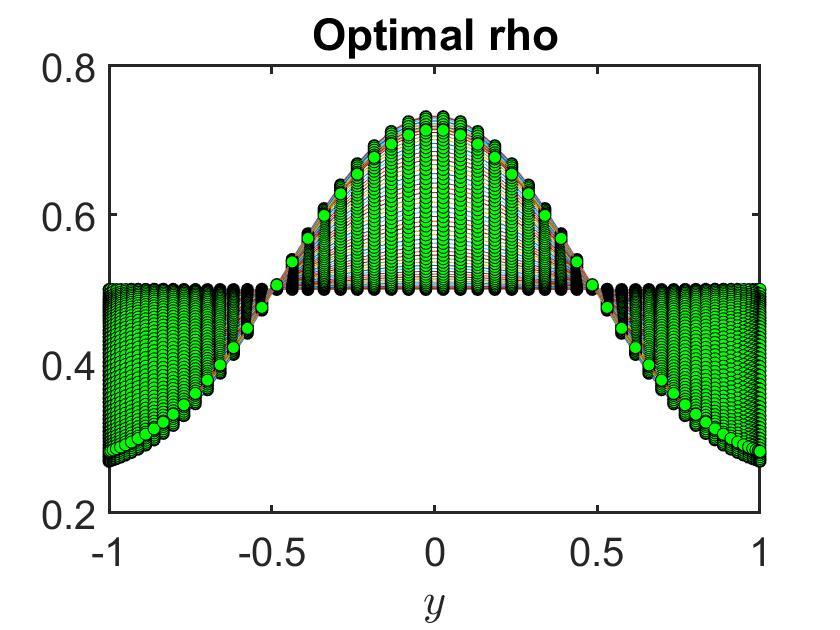
\includegraphics[scale=0.3]{rhoOptM2.jpg}
	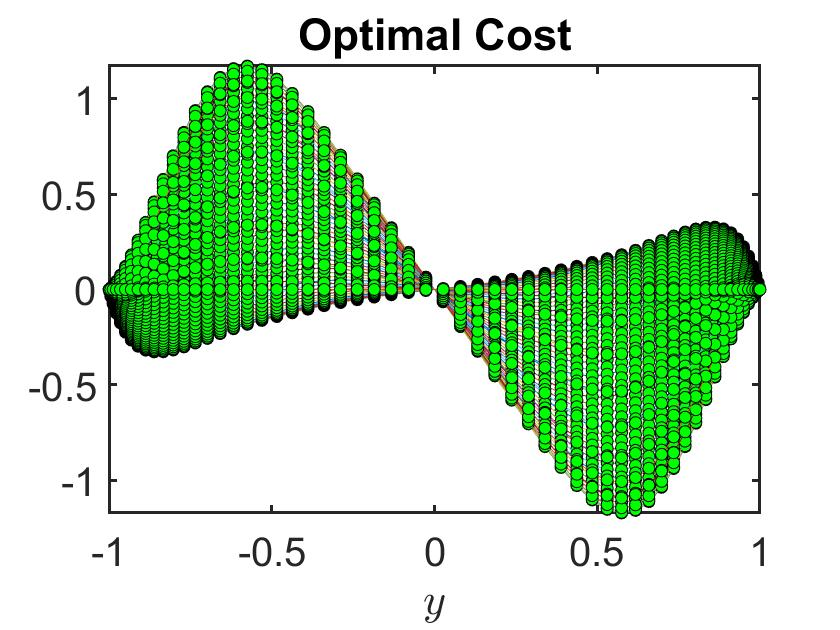
\includegraphics[scale=0.3]{wOptM2.jpg}
	\caption{Solutions $\rho_{FW}$ and $\rho_{Opt}$ and Optimal control $w$, $\gamma = - 1$, $\beta = 10^{-3}$, with $D_0 = 1$.}
	\label{rhoM1}
\end{figure}
\begin{figure}[h]
	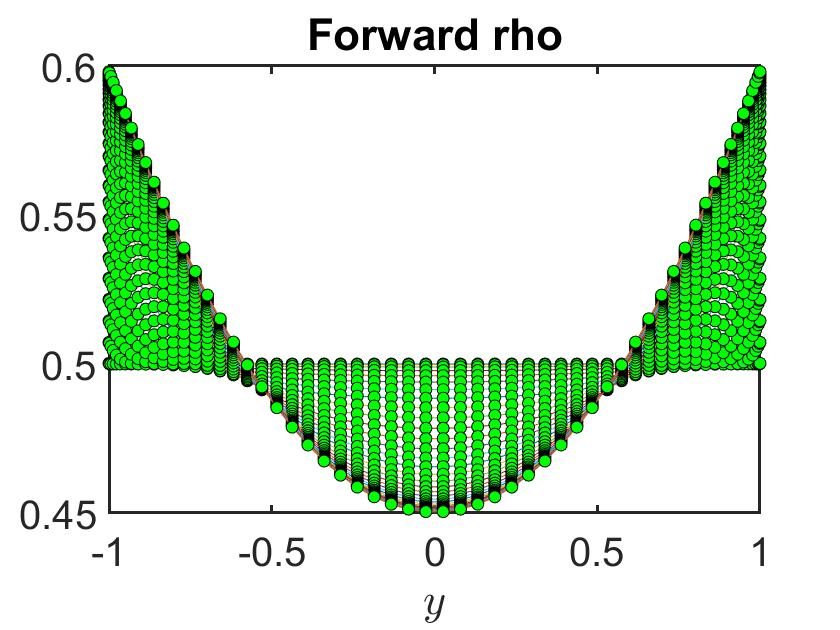
\includegraphics[scale=0.3]{rhoFWM3.jpg}	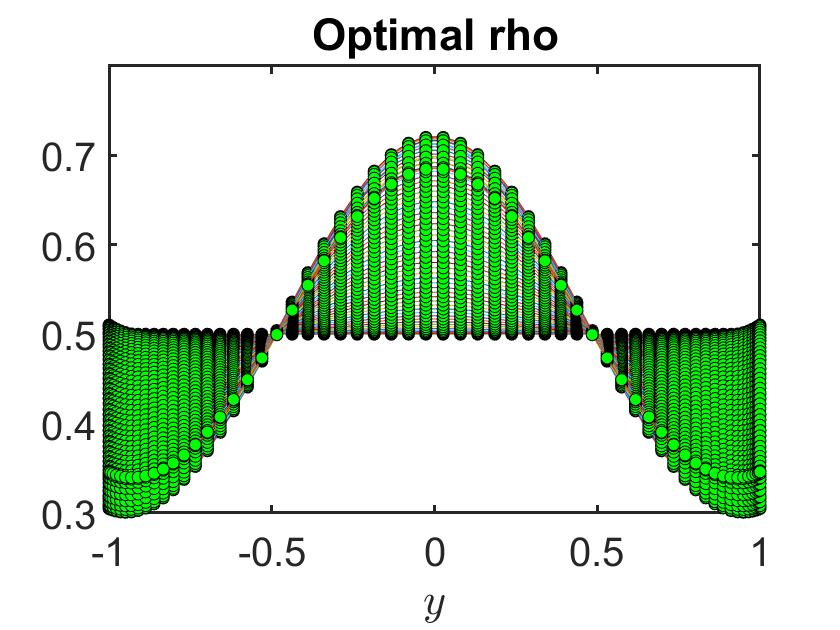
\includegraphics[scale=0.3]{rhoOptM3.jpg}
	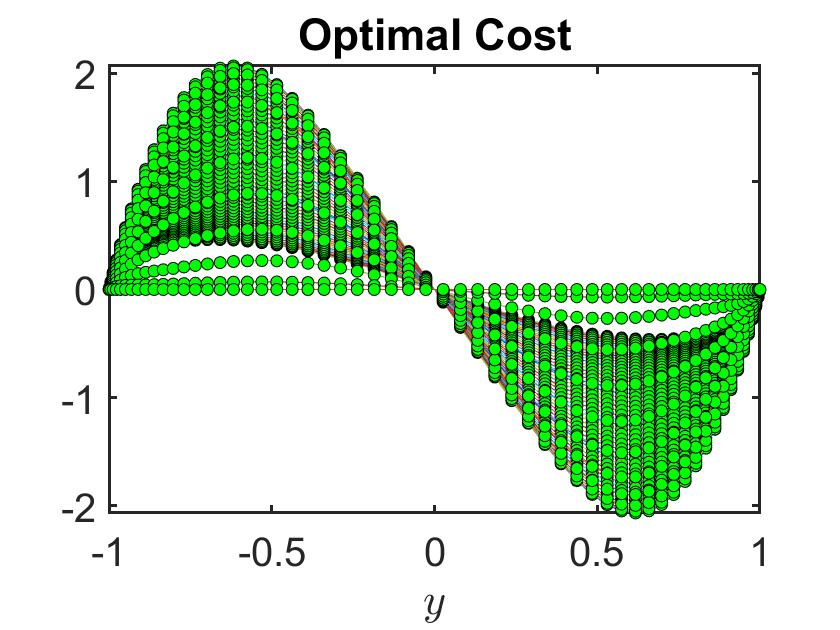
\includegraphics[scale=0.3]{wOptM3.jpg}
	\caption{Solutions $\rho_{FW}$ and $\rho_{Opt}$ and Optimal control $w$, $\gamma = 1$, $\beta = 10^{-3}$, with $D_0 = 1$.}
	\label{rhoM2}
\end{figure}
\subsection{Diffusion vs advection term}
Setting $D_0=2$, $\beta = 10^{-3}$ and $\gamma = -1$ converges. This again suggests that the diffusion advection interaction is influencing the stability of the code.


\section{Interacting Problems - moving target 2}
The target is now
\begin{align*}
\hat \rho = (1-t)0.5 + t\frac{1}{4}(\cos(\pi y + \pi) + 2),
\end{align*}
see Figure \ref{rhoHat4}.
\begin{figure}[h]
	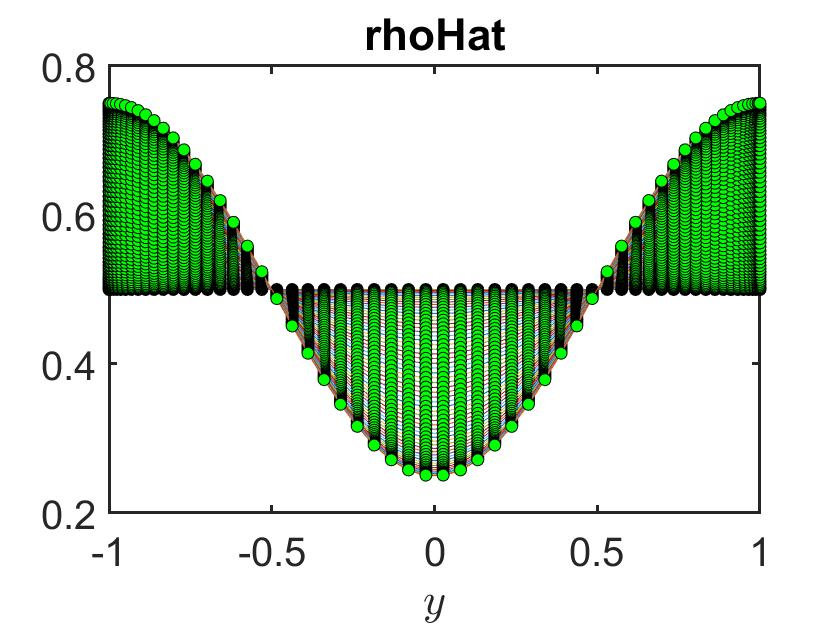
\includegraphics[scale=0.3]{rhoHat4.jpg}
	\caption{Moving target 2.}
	\label{rhoHat4}
\end{figure}

First try $\beta = 10^{-1}$, $\gamma = 1$, which converges in $651$ iterations, $J_{FW} = 0.0047$, $J_{Opt} = 0.0040$. Then choosing $\gamma = -1$, converges with $J_{FW} = 0.0209$ and $J_{Opt} = 0.0168$.\\
Try $\beta = 10$, converges for both $\gamma =1$, $\gamma = -1$, $J_{FW}$ and $J_{Opt}$ basically identical. As perhaps expected, $\beta = 10^3$ converges within one iteration for both choices of $\gamma$.\\
Try $\beta = 10^{-3}$ and $\gamma = 1$. This converges in $625$ iterations, $J_{FW} = 0.0047$ and $J_{Opt} = 3.4051 \times 10^{-4}$, see Figure \ref{rhot1}.
Looking at $\gamma = -1$, this converges as well, $J_{FW} = 0.0209$, $J_{Opt} = 8.9783 \times 10^{-4}$, see Figure \ref{rhot2}. One question is now why this works for this example, but not for the one above, given that they are very similar in nature.\\

Test $\beta = 10^{-3}$, $\gamma = -1$ with Picard. It converges in $619$ iterations but is considerably slower than FixPt. $J_{FW} = 0.0209$ and $J_{Opt} = 8.9784 \times 10^{-4}$ are basically the same values as with FixPt. For $\gamma = 1$ it also converges and we have $J_{FW} = 0.0047$ and $J_{Opt} = 3.4041 \times 10^{-4}$, which is again very close to the values with FixPt.

\begin{figure}[h]
	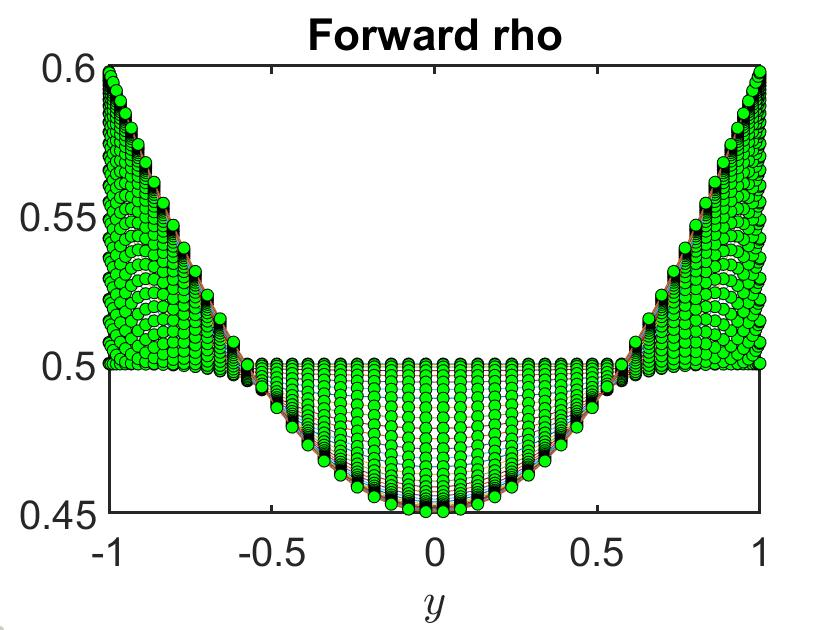
\includegraphics[scale=0.3]{rhoFWt.jpg}	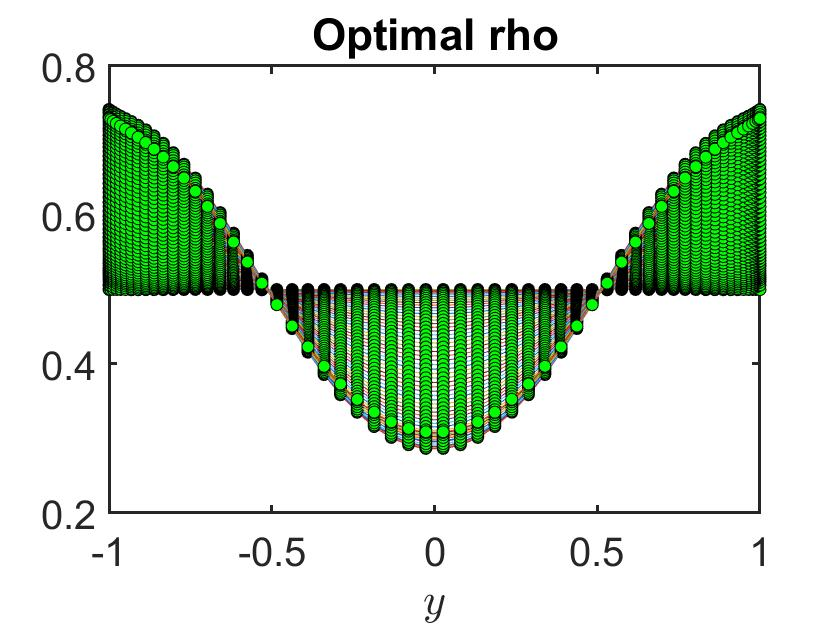
\includegraphics[scale=0.3]{rhoOptt.jpg}
	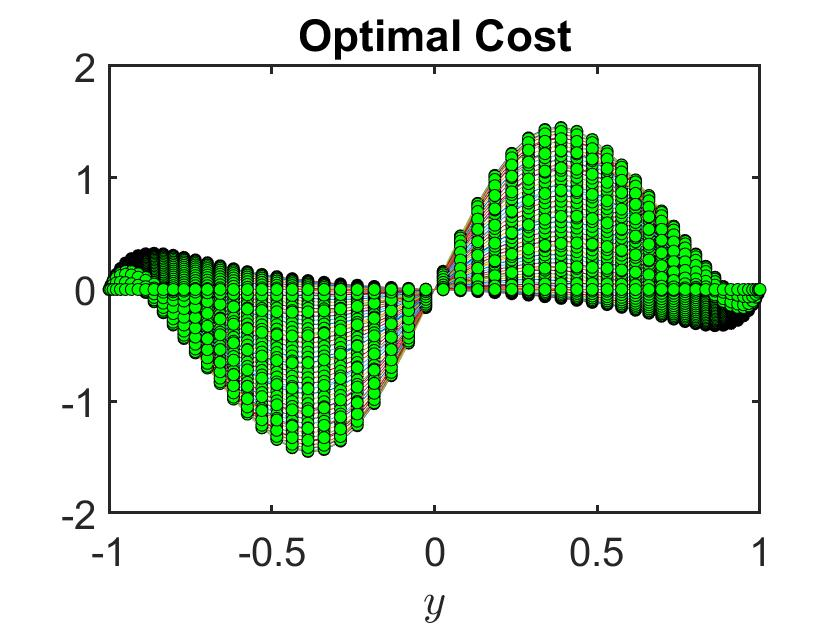
\includegraphics[scale=0.3]{wOptt.jpg}
	\caption{Solutions $\rho_{FW}$ and $\rho_{Opt}$ and Optimal control $w$, $\gamma = 1$, $\beta = 10^{-3}$, with $D_0 = 1$.}
	\label{rhot1}
\end{figure}


\begin{figure}[h]
	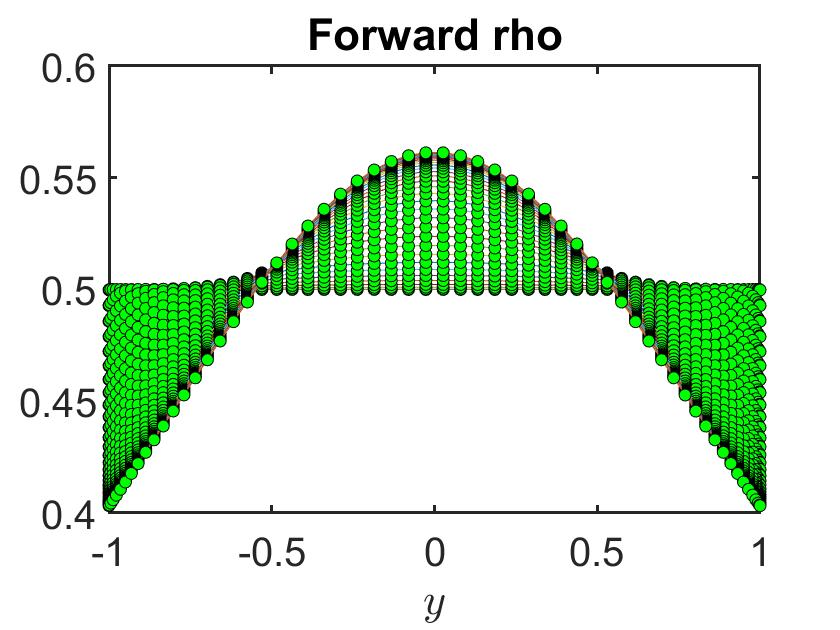
\includegraphics[scale=0.3]{rhoFWt2.jpg}	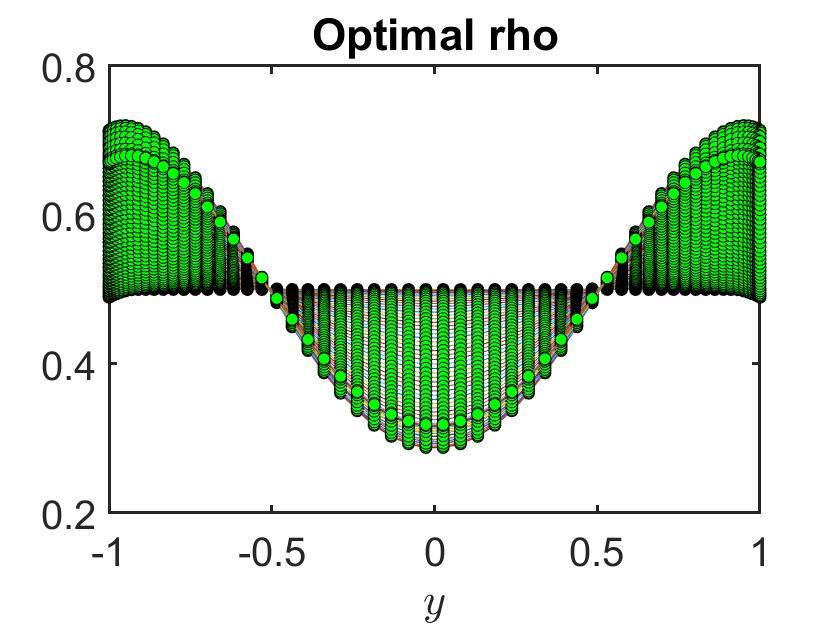
\includegraphics[scale=0.3]{rhoOptt2.jpg}
	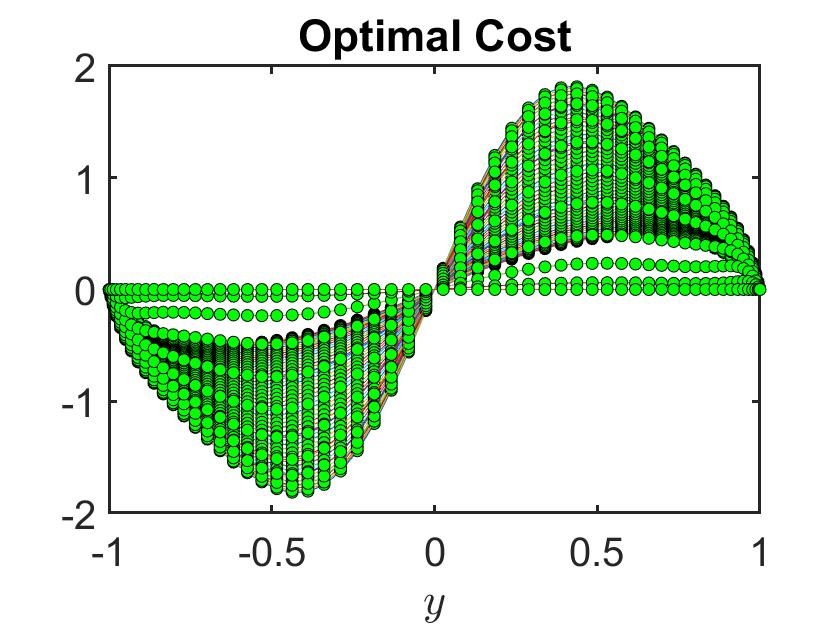
\includegraphics[scale=0.3]{wOpt2.jpg}
	\caption{Solutions $\rho_{FW}$ and $\rho_{Opt}$ and Optimal control $w$, $\gamma = -1$, $\beta = 10^{-3}$, with $D_0 = 1$.}
	\label{rhot2}
\end{figure}
\subsection{Diffusion vs advection term}
We can try to break this example by decreasing the diffusion coefficient.
Choosing $\gamma = 1$, since this works in the same direction as the advection. Interestingly, I can lower the diffusion coefficient to $D_0 = 0.17$ and the algorithm converges. At $D_0 = 0.16$ it diverges in $4$ Iterations.
$D_0 = 0.1699$ diverges at a consistency of $0.00011768$ in $474$ iterations, see Figure \ref{rhoDiv1} and compare to the case with $D_0=1$ in Figure \ref{rhot1}. In Figure \ref{rhoDiv1} the optimal cost is of order $0.5$, while in Figure \ref{rhot1} the cost is of order $2$.
Already at $D_0 = 0.01695$, the algorithm diverges in $9$ iterations. \\
Trying to break $\gamma = -1$ seems to be easier. Choosing $D_0 =0.5$, the algorithm diverges at $0.00271887$ in $342$ iterations, however $D_0 =0.51$ converges.
\begin{figure}[h]
	\includegraphics[scale=0.3]{rhoFWDiv1.jpg}	\includegraphics[scale=0.3]{rhoOptDiv1.jpg}
	\includegraphics[scale=0.3]{wOptDiv1.jpg}
	\caption{Solutions $\rho_{FW}$ and $\rho_{Opt}$ and Optimal control $w$, $\gamma = 1$, $\beta = 10^{-3}$, with $D_0 = 0.1699$.}
	\label{rhoDiv1}
\end{figure}
	
	
	
\section{$\gamma = 0$ case}
As a comparison, this is moving target $1$ with $\gamma =0$ and $\beta = 10^{-3}$, see Figure \ref{rhog1}. $J_{FW} = 0.0104$, $J_{Opt} = 5.4136 \times 10^{-4}$. $\gamma = -1$ gives lower $J$, $\gamma = 1$ higher $J$.
\begin{figure}[h]
	\includegraphics[scale=0.3]{rhoOptg1.jpg}
	\includegraphics[scale=0.3]{wOptg1.jpg}
	\caption{Solution $\rho_{Opt}$ and Optimal control $w$, $\gamma = 0$, $\beta = 10^{-3}$, with $D_0 = 1$.}
	\label{rhog1}
\end{figure}
	
This is moving target $2$ with $\gamma =0$ and $\beta = 10^{-3}$, see Figure \ref{rhog2}. $J_{FW} = 0.0104$, $J_{Opt} = 5.4136 \times 10^{-4}$. $\gamma =1$ gives lower $J$, $\gamma = -1$ higher $J$, which is the opposite of the problem with moving target $1$ and absolutely expected.
	\begin{figure}[h]
		\includegraphics[scale=0.3]{rhoOptg2.jpg}
		\includegraphics[scale=0.3]{wOptg2.jpg}
		\caption{Solution $\rho_{Opt}$ and Optimal control $w$, $\gamma = 0$, $\beta = 10^{-3}$, with $D_0 = 1$.}
		\label{rhog2}
	\end{figure}
	
\end{document}